
\documentclass{beamer}
\usetheme{metropolis}
\usepackage{hyperref}
\begin{document}
\title{NEAT and HyperNEAT}
\author{Michal Pospěch \& Daniel Crha}
\date{\today}
\institute{Faculty of Mathematics and Physics, Charles University}

\maketitle
\section{Neuroevolution}
\begin{frame}{Fixed Topology Evolution}
    \begin{itemize}
        \item Searching the space of connection weights
        \item Topology is given, does not change during evolution
    \end{itemize}

\end{frame}
\begin{frame}{Evolving Topology}
    \begin{itemize}
        \item Technical challenges:
              \begin{itemize}
                  \item good representation
                  \item not removing non-optimized network to early
                  \item minimisation of networks without need for a complexity function
              \end{itemize}
        \item TWEANNs - Topology and Weight Evolving Artificial Neural Networks
    \end{itemize}

\end{frame}
\section{NEAT}
\begin{frame}{NEAT}
    \begin{itemize}
        \item NeuroEvolution of Augmenting Topologies
        \item Stanley and Miikkulainen, 2002
        \item solves all the issues aforementioned issues
    \end{itemize}
\end{frame}
\begin{frame}{Encoding and Mutation}
    \begin{columns}
        \begin{column}{0.5\textwidth}
            \begin{itemize}
                \item  linear representations of network connectivity
                      \begin{itemize}
                          \item 2 types of genes (nodes and connections)
                          \item innovation number
                          \item node
                      \end{itemize}
                \item 3 types of mutation
                      \begin{itemize}
                          \item connection weight mutation
                          \item new node
                          \item new connection
                      \end{itemize}
            \end{itemize}
        \end{column}
        \begin{column}{0.5\textwidth}
            \begin{figure}[c]
                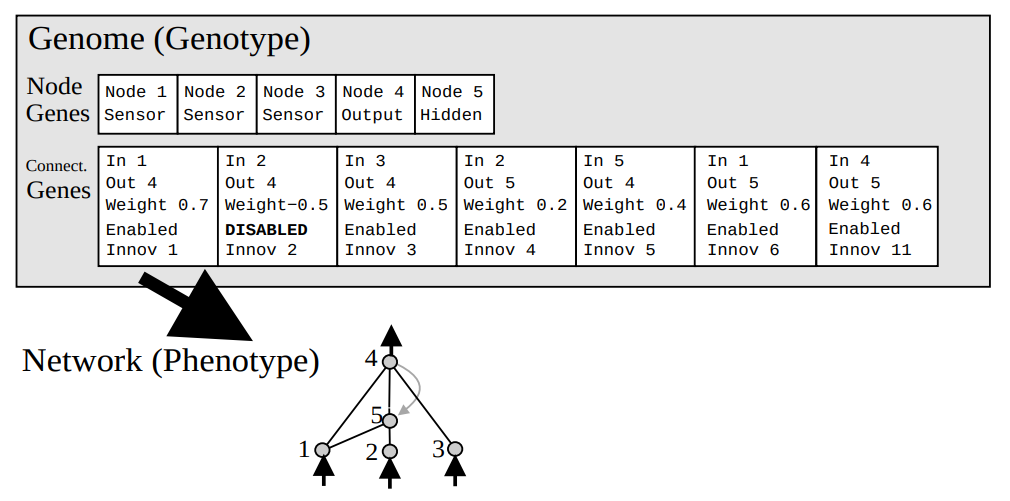
\includegraphics[width = \textwidth]{img/encoding.png}
            \end{figure}
            \begin{figure}[c]
                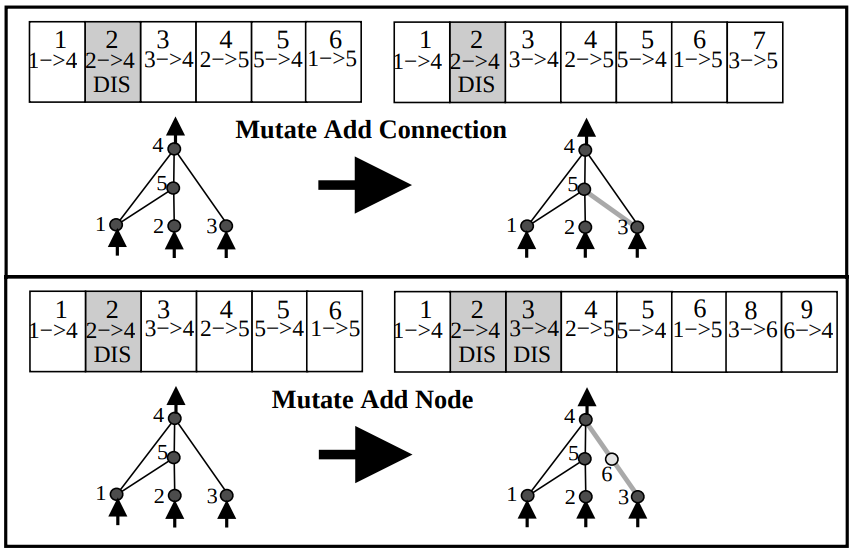
\includegraphics[width = \textwidth]{img/mutation.png}
            \end{figure}
        \end{column}
    \end{columns}
\end{frame}
\begin{frame}{Historical Markings and Crossover}
    \begin{itemize}
        \item innovation number
              \begin{itemize}
                  \item new gene via mutation \textrightarrow\ global innovation number++
                  \item used to line-up genomes during crossover
              \end{itemize}
        \item crossover
              \begin{itemize}
                  \item matching genes randomly
                  \item all disjoint and excess genes
              \end{itemize}
    \end{itemize}
\end{frame}
\begin{frame}{Crossover}
    \begin{figure}[c]
        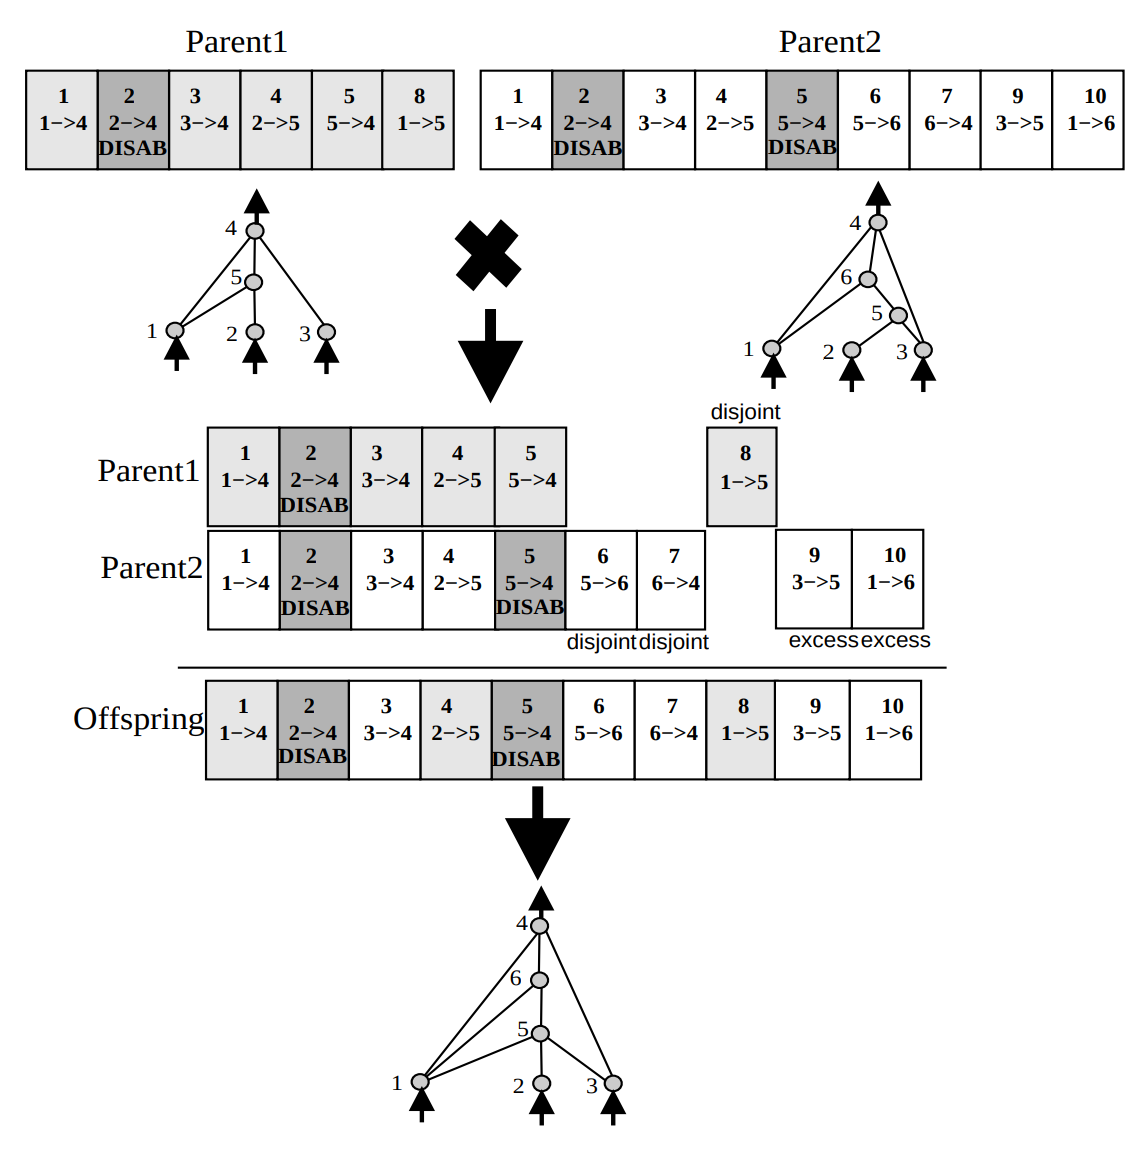
\includegraphics[scale=0.2]{img/crossover.png}
    \end{figure}
\end{frame}
\begin{frame}{Speciation}
    \begin{itemize}
        \item population is divided into species based on compatibility history \begin{equation*}
                  \delta = \frac{c_1E}{N}+\frac{c_2D}{N}+c_3 \overline{W}
              \end{equation*} and compatibility threshold $\delta_t$
        \item each population is assigned number of offsprings based on sum of its \emph{adjusted} fitnesses
              \begin{equation*}
                  f_i' =\frac{f_i}{\sum_{j=1}^n sh(\delta(i,j))}
              \end{equation*}
        \item novel topologies are protected from extinction
    \end{itemize}
\end{frame}
\section{HyperNEAT}
\begin{frame}{Compositional Pattern Producing Networks}
    \begin{columns}
        \begin{column}{0.5\textwidth} \begin{itemize}
                \item represent repeating patterns in cartesian space
                \item nodes are functions
                \item simple functions can be composed into networks producing complex patterns (repetition, symmetry)           \end{itemize}\end{column}
        \begin{column}{0.5\textwidth}
            \begin{figure}[c]
                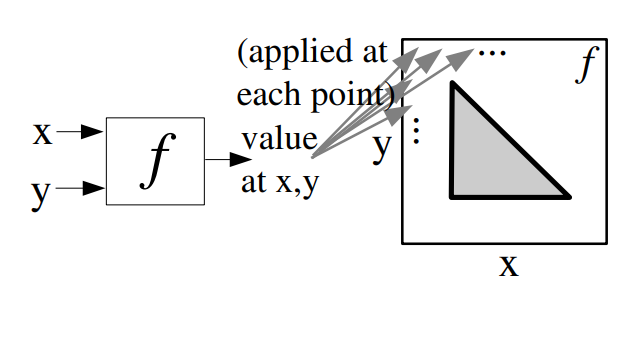
\includegraphics[width=\textwidth]{img/function.png}
            \end{figure}
            \begin{figure}[c]
                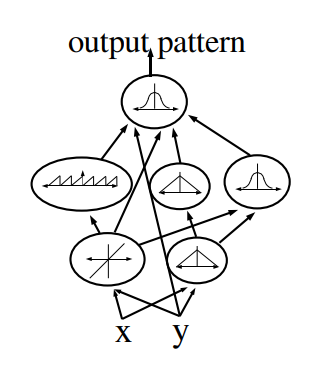
\includegraphics[width=0.6\textwidth]{img/CPNN.png}
            \end{figure}
        \end{column}
    \end{columns}
\end{frame}
\begin{frame}{HyperNEAT}
    \begin{columns}
        \begin{column}{0.5\textwidth}
            \begin{itemize}
                \item CPPNs evolved via NEAT
                \item nodes are given (2D grid)
                \item input: 2 points , output: weight of connection
            \end{itemize}
        \end{column}
        \begin{column}{0.5\textwidth}
            \begin{figure}[c]
                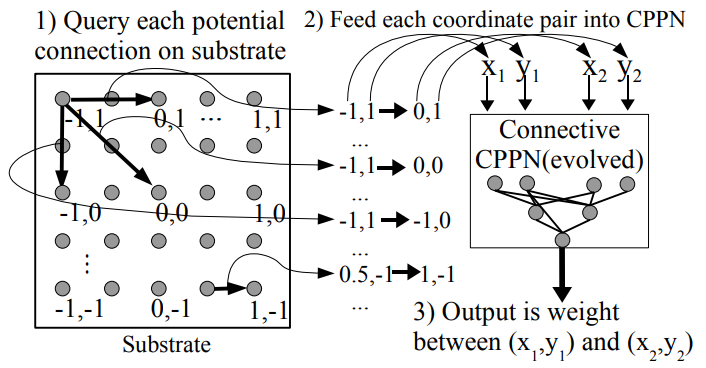
\includegraphics[width=\textwidth]{img/HyperNEAT.png}
            \end{figure}
        \end{column}
    \end{columns}
\end{frame}
\begin{frame}{Substrate}
    \begin{itemize}
        \item types
              \begin{itemize}
                  \item 2D grid
                  \item 3D grid
                  \item sandwich (\emph{state-space sandwich})
                  \item circular
              \end{itemize}
        \item placement of inputs and outputs can be exploited
        \item can be up/down-scaled
    \end{itemize}
\end{frame}
\section{Performance and examples}
\begin{frame}{Evaluation}
    \begin{itemize}
        \item used environment - \href{https://gym.openai.com}{OpenAI Gym, Cartpole-v1}
        \item our results (GIFs) - \href{https://imgur.com/a/4nLJ4oV}{https://imgur.com/a/4nLJ4oV}
        \item other methods - \href{https://github.com/adibyte95/CartPole-OpenAI-GYM}{https://github.com/adibyte95/CartPole-OpenAI-GYM}
    \end{itemize}
\end{frame}
\begin{frame}{NEAT and cartpole}
    \begin{figure}[c]
        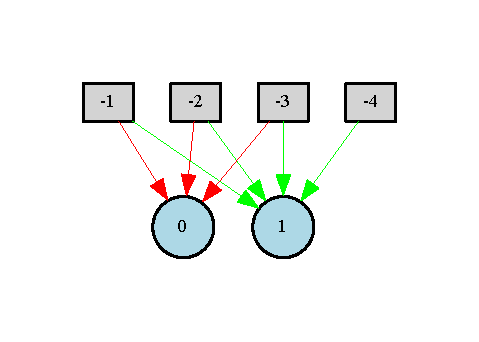
\includegraphics[width=\textwidth]{pdf/neat_pole_balancing_winner.pdf}
    \end{figure}
\end{frame}
\begin{frame}{HyperNEAT and cartpole}
    \begin{columns}
        \begin{column}{0.5\textwidth}
            \begin{figure}[c]
                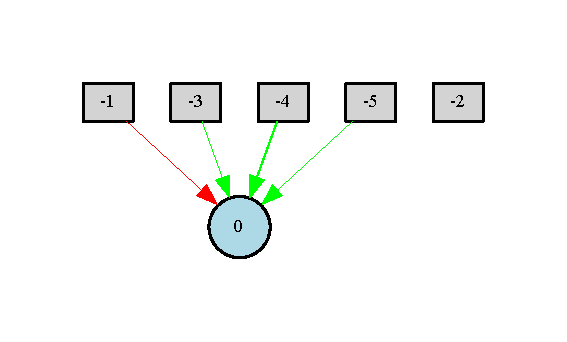
\includegraphics[width=\textwidth]{pdf/hyperneat_pole_balancing_cppn.pdf}
                \caption{CPPN}
            \end{figure}\end{column}
        \begin{column}{0.5\textwidth}
            \begin{figure}[c]
                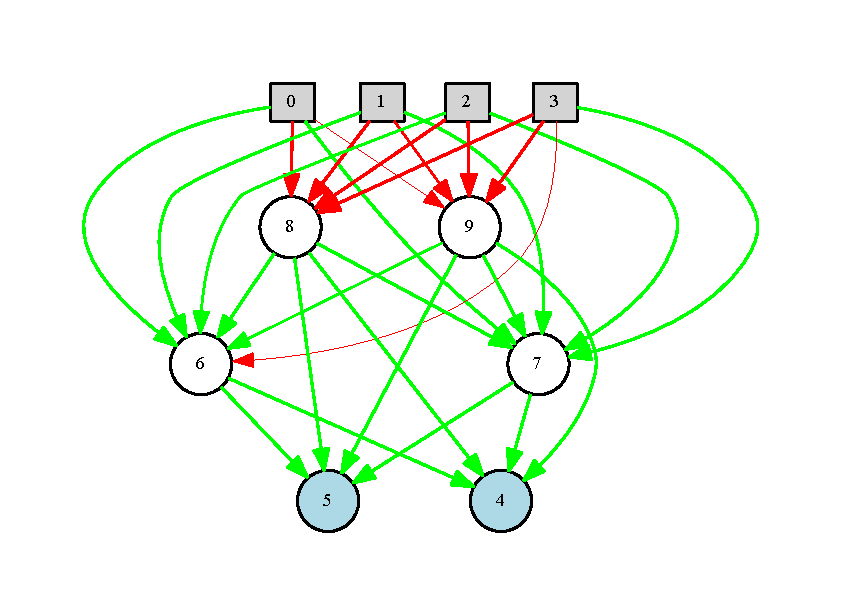
\includegraphics[width=\textwidth]{pdf/hyperneat_pole_balancing_winner.pdf}
                \caption{ANN}
            \end{figure}
        \end{column}
    \end{columns}
\end{frame}
\begin{frame}{Comparison}
    \begin{columns}
        \begin{column}{0.5\textwidth}
            \begin{figure}[c]
                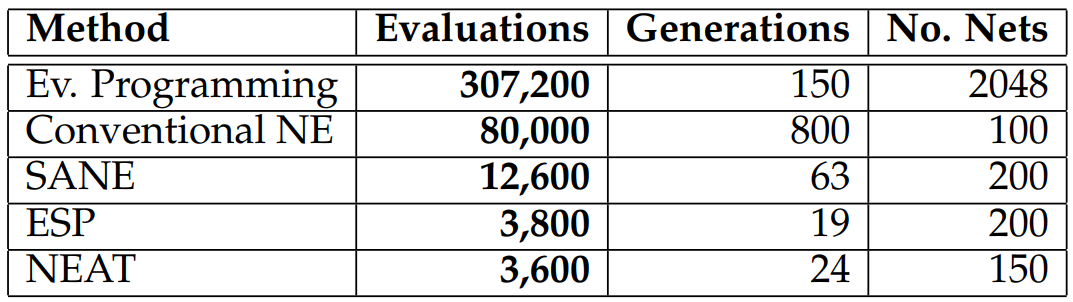
\includegraphics[width=\textwidth]{img/pole_balancing_table.png}
                \caption{Pole balancing results}
            \end{figure}\end{column}
        \begin{column}{0.5\textwidth}
            \begin{figure}[c]
                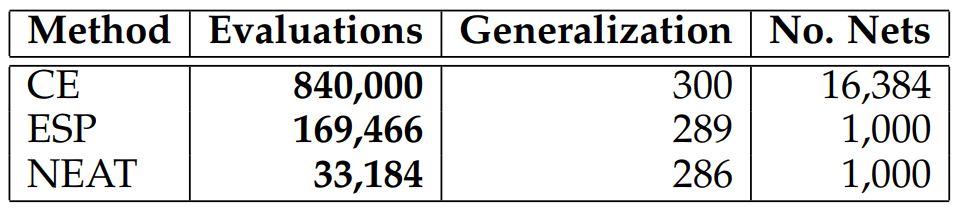
\includegraphics[width=\textwidth]{img/double_pole_balancing_table.png}
                \caption{Double pole balancing results}
            \end{figure}
        \end{column}
    \end{columns}
\end{frame}
\end{document}
